\documentclass[dvipdfmx,14pt]{beamer}
\usepackage{lipsum}
\usetheme{Verona}
\usepackage{bxdpx-beamer}
\usepackage{pxjahyper}
\usepackage{minijs}
\usepackage{mathpazo}
\usepackage{amsmath,amssymb}
\usepackage{graphicx}
\graphicspath{{fig_tab/os20221215/}}
\usepackage{array}
\usepackage{tikz}
\usepackage{wrapfig}
\usepackage{float}
\usepackage{here}
\usepackage{lscape}
\usepackage{ascmac}
\usepackage{tabularx}
\renewcommand{\kanjifamilydefault}{\gtdefault}
\hypersetup{% hyperrefオプションリスト
 setpagesize=false,
 bookmarksnumbered=true,%
 bookmarksopen=true,%
 colorlinks=true,%
 linkcolor=blue,
 citecolor=blue,
 urlcolor = magenta
}
\setbeamertemplate{navigation symbols}{}

\title[Currie, Voorheis, and Walker, Forthcoming]{What Caused Racial Disparities \\ in Particulate Exposure to Fall? \\ New Evidence from the Clean Air Act \\ and Satellite-Based Measures of Air Quality}
\subtitle{Currie, Voorheis, and Walker (AER, Forthcoming)}
\author{Reviewed by R. TANJI}
\date[12/15/2022 OS Semi.]{December 15th, 2022 \\ Ohtake-Sasaki Seminar}
\institute[]{Osaka University, Graduate School of Economics}

\begin{document}

\begin{frame}\frametitle{}
\titlepage
\end{frame}

\section{Introduction}

\begin{frame}\frametitle{Abstract}
  \begin{itemize}
    \item This paper examines the underlying structure that causes racial differences in exposure to ambient air pollution in the United States.
    \begin{itemize}
      \item The difference have declined significantly over the past 20 years.
    \end{itemize}
    \item Clean Air Act (CAA) explains the excess convergence in Black-White pollution exposure
    \begin{itemize}
      \item Areas with larger Black populations saw greater CAA-related declines in PM2.5 exposure
      \item Over 60\% of the reduction in the racial convergence in PM2.5 pollution exposure since 2000
    \end{itemize}
  \end{itemize}
\end{frame}

\frame{\tableofcontents}

\begin{frame}{Literature}
  \begin{itemize}
    \item The existing evidence about racial disparities in pollution exposure is largely piecemeal and indirect.
    \begin{itemize}
      \item Low income and/or racial minorities in the U.S. have been exposed to environmental burdens (Office, 1983; Chavis and Lee, 1987)
      \item Lack of monitoring device to track small particulates (Fowlie, Rubin, and Walker, 2019)
      \item Alternative measurement: distance to a polluting facility
    \end{itemize}
    \item Moreover, we know very little about why racial gaps in pollution exposure may have changed over time.
  \end{itemize}
\end{frame}

\begin{frame}{}
  \begin{figure}
    \centering
    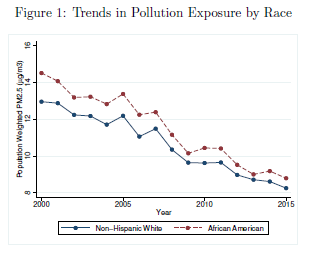
\includegraphics[scale = .5]{F1.png}
    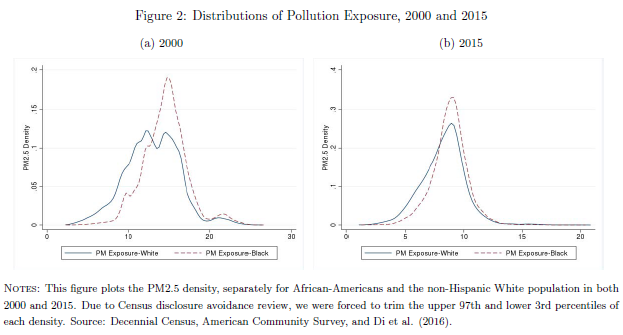
\includegraphics[scale = .5]{F2.png}
  \end{figure}
\end{frame}

\section{Data}
\frame{\sectionpage}
\begin{frame}{}

\end{frame}

\section{Decomposing Differences in Pollution Exposure}
\frame{\sectionpage}
\begin{frame}{}
  
\end{frame}

\section{The Clean Air Act and Relative Changes in Pollution Exposure}
\frame{\sectionpage}
\begin{frame}{}
  
\end{frame}

\section{Conclusion}
\frame{\sectionpage}
\begin{frame}{}
  
\end{frame}

\end{document}
